In this section, the basic GeoPAT procedures are presented. These are: 

\begin{itemize}
	\item {\bf Search} - search for areas similar to a query
	\item {\bf Change detection} - comparison of local patterns between two maps
	\item {\bf Segmentation} - division of a map into regions of cohesive patterns
	\item {\bf Clustering} - grouping patterns that are similar to each other
\end{itemize}

The procedures are explained using the workflow schemes and examples.
All of the examples how to process categorical data are shown on a $42\times 69$ km ($1400\times 2300$ px) part of the National Land Cover Dataset (NLCD) covering area around the city of Augusta, GA (Figure \ref{FIG:AUGUSTA}).
This area is characterized by high diversity of land cover categories and patterns.
Thus it is perfect for various pattern analyzes.

\begin{figure}[H]
	\centering
	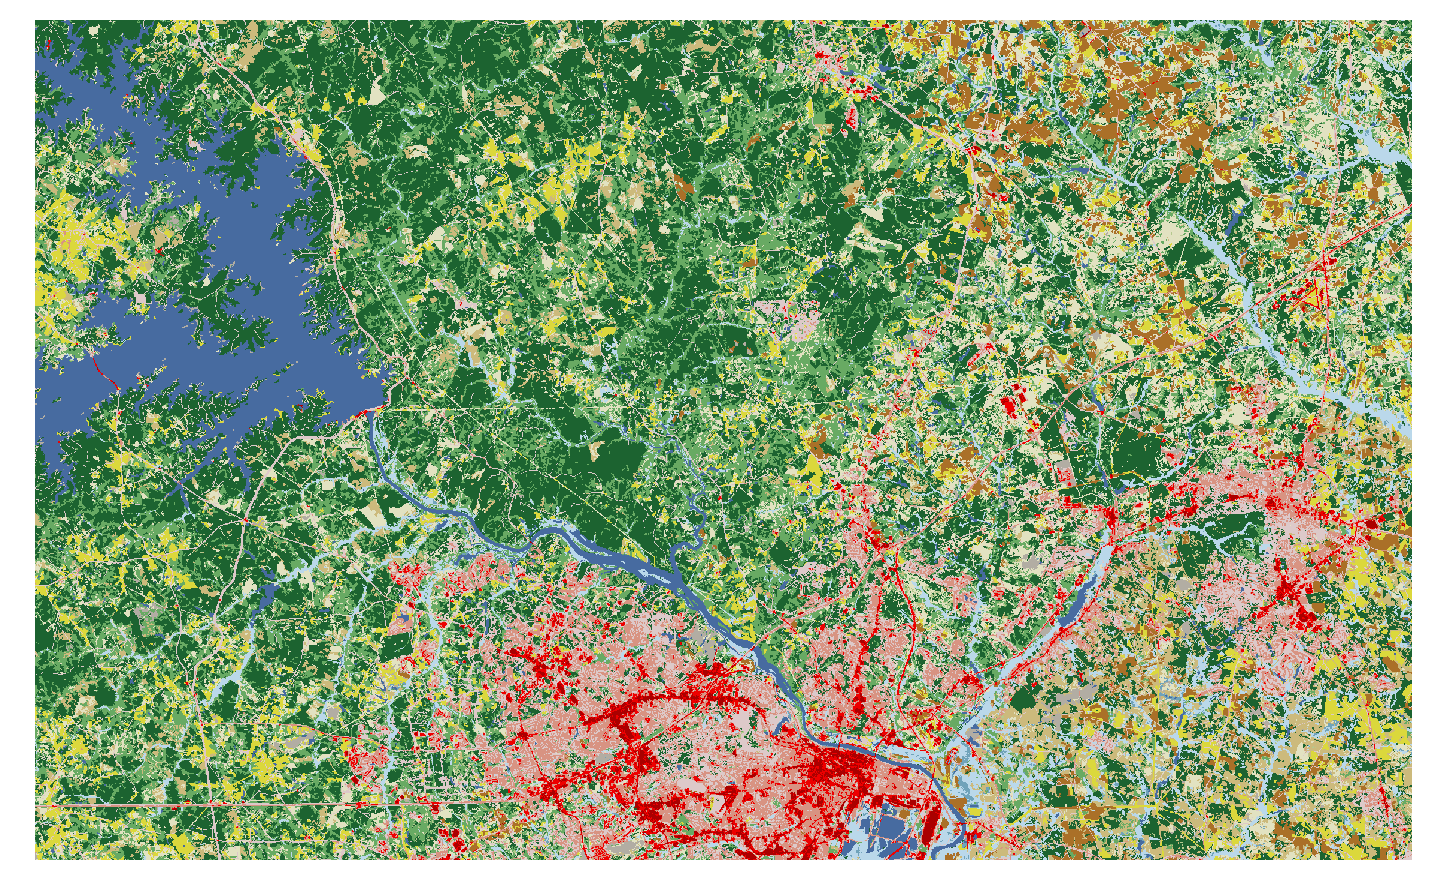
\includegraphics[width=\textwidth]{atlanta.png}
	\caption{Part of NLCD, covering area around Augusta, GA used in the examples}
	\label{FIG:AUGUSTA}
\end{figure}

\FloatBarrier

\subsection{Search}

Search functionality enables user to produce maps of similarity. 
These maps show the level of similarity between a specified motifel (query) and a grid of motifels.
The input is one or more GeoTIFF raster maps (depending on a data and signature type; see appendix \ref{signatures} for more information), and XY coordinates of one or more points in space.
The result is one or more GeoTIFF raster maps which have the same extent as the grid of motifels specified by user.
The number of resulting maps is the same as the number of points provided.
The workflows for categorical and time series maps differ.

\subsubsection{Search on categorical maps}
Figure \ref{FIG:SEARCH} presents general workflow path for producing similarity maps using a categorical raster data. 

\begin{figure}[H]
	\centering
	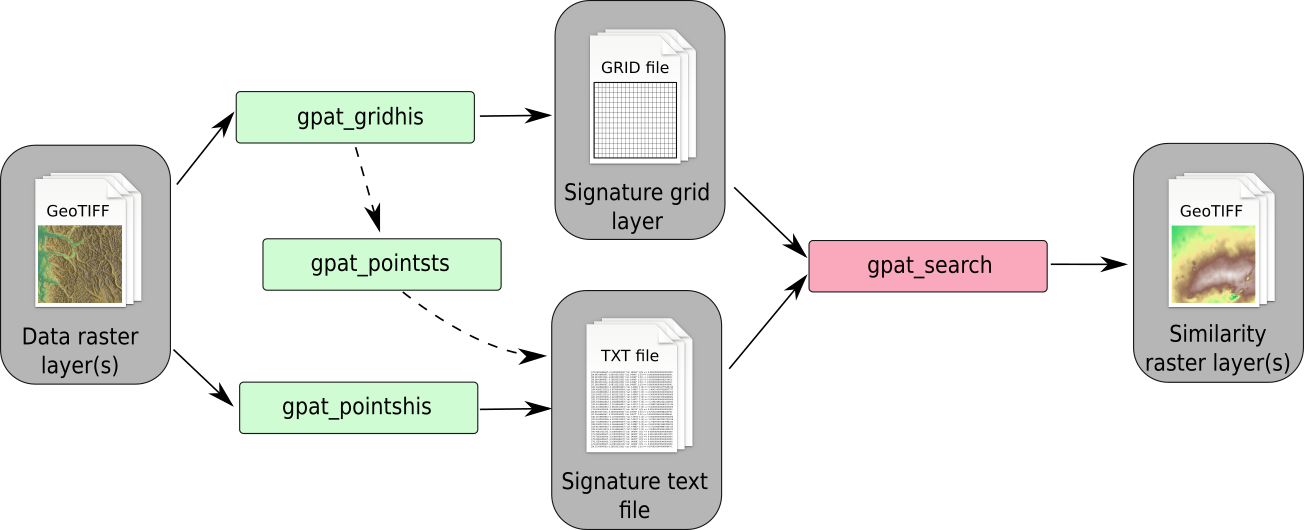
\includegraphics[width=\textwidth]{search_scheme.png}
	\caption{Workflow path for search on categorical maps}
	\label{FIG:SEARCH}
\end{figure}

The first step is to prepare signature files for both, query motifels and grid of motifels, using two separate modules, {\it gpat\_pointshis} and {\it gpat\_gridhis} respectively. 
The second step is to use these signature files as inputs to {\it gpat\_search} module in order to the produce similarity maps.\\\\
{\bf Example:}

\begin{minipage}{\linewidth}
\begin{lstlisting}
gpat_gridhis -i Augusta2011.tif -o grid -s cooc -z 50 -f 50 -n pdf
gpat_pointshis -i Augusta2011.tif -o query_signatures.txt -s cooc -z 50 -n pdf --xy_file=coordinates.txt
gpat_search -i grid -r query_signatures.txt
\end{lstlisting}
\end{minipage}

\begin{figure}[H]
	\centering
	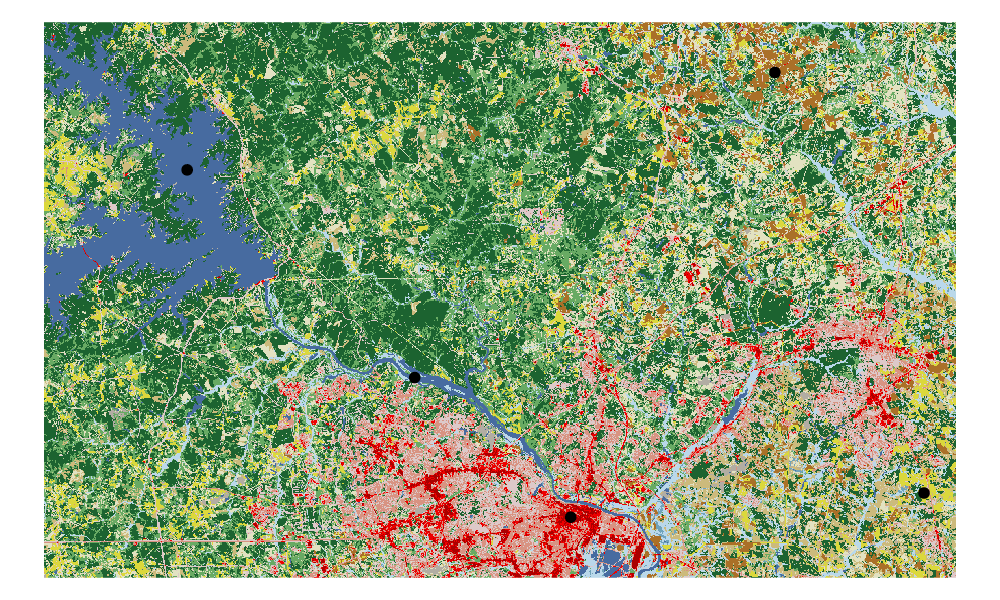
\includegraphics[width=\textwidth]{searchhis_plot1.png}
	\caption{Points of interest on the top of a landcover map}
	\label{FIG:SEARCH1}
\end{figure}

\begin{figure}[H]
	\centering
	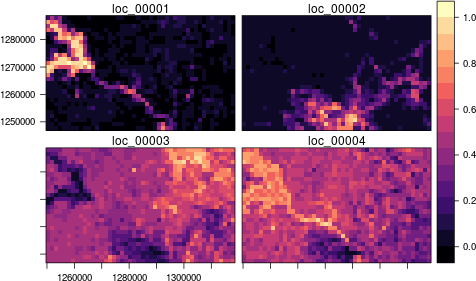
\includegraphics[width=\textwidth]{searchhis_plot2.png}
	\caption{Output similarity maps}
	\label{FIG:SEARCH2}
\end{figure}

\FloatBarrier

\subsubsection{Search on time series}
TODO
\begin{figure}[H]
	\centering
	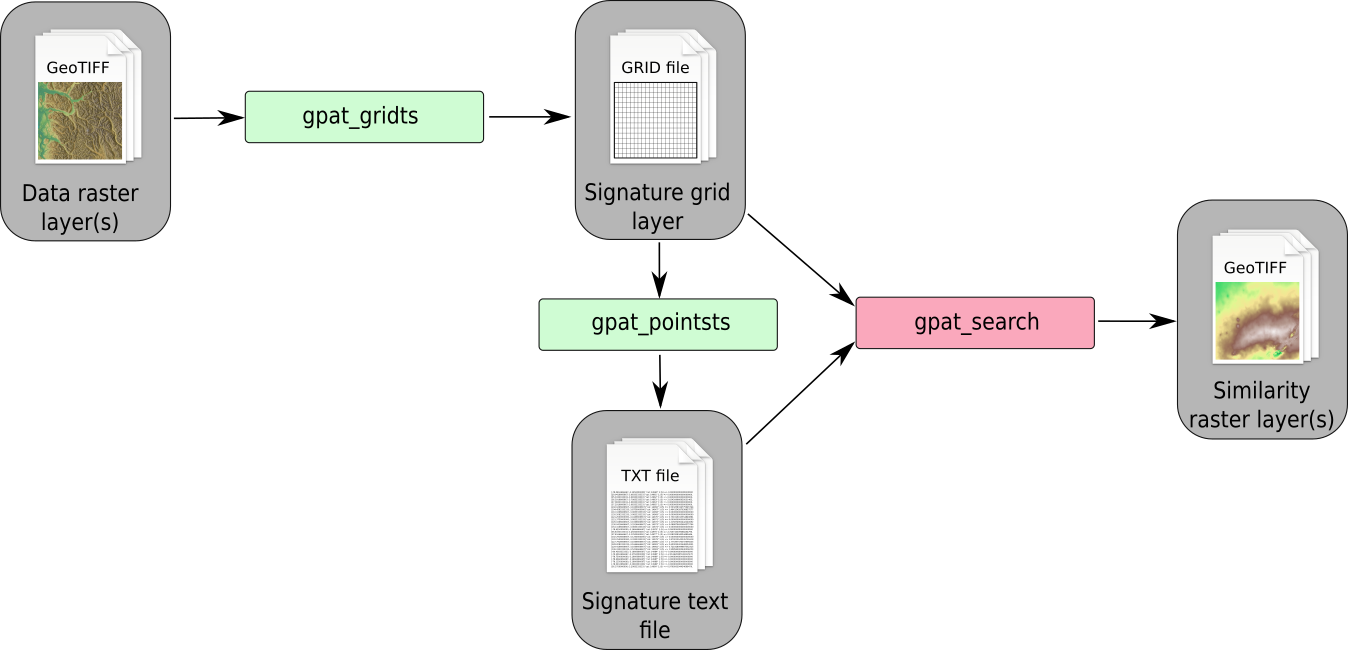
\includegraphics[width=\textwidth]{searchts_scheme.png}
	\caption{Workflow path for search on time series.}
	\label{FIG:SEARCHTS}
\end{figure}

% \begin{minipage}{\linewidth}
% \begin{lstlisting}
% gpat_pointsts -i grid -o query_signatures.txt --xy_file=coordinates.txt
% \end{lstlisting}
% \end{minipage}

\FloatBarrier

\subsection{Change detection}
TODO
\begin{figure}[H]
	\centering
	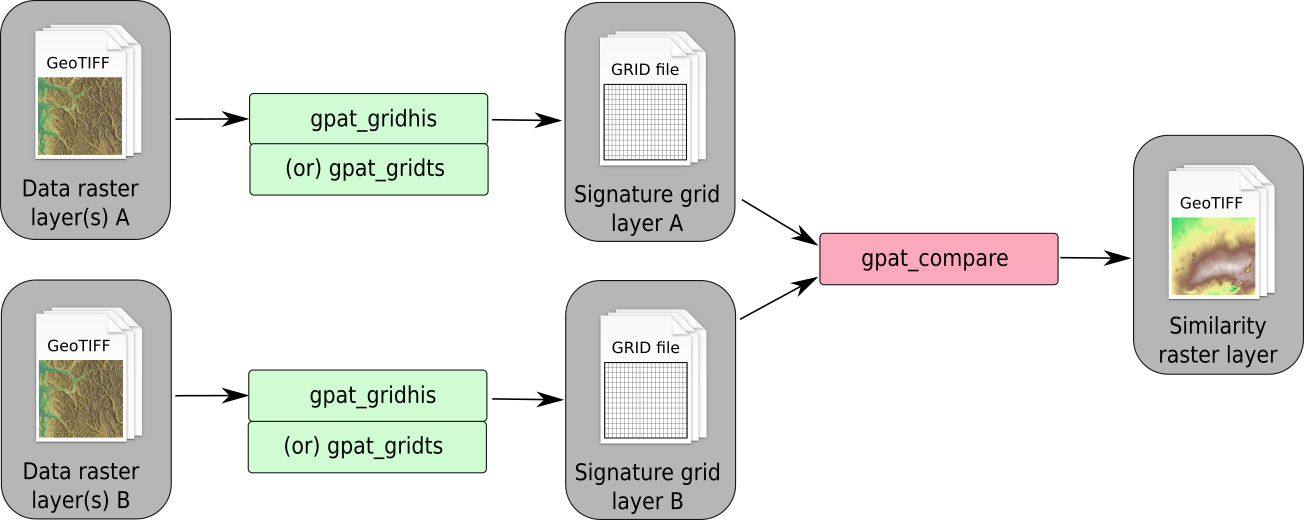
\includegraphics[width=\textwidth]{compare_scheme.png}
	\caption{Workflow path for change detection.}
	\label{FIG:CHANGE}
\end{figure}

\FloatBarrier

\subsection{Segmentation}
TODO
\begin{figure}[H]
	\centering
	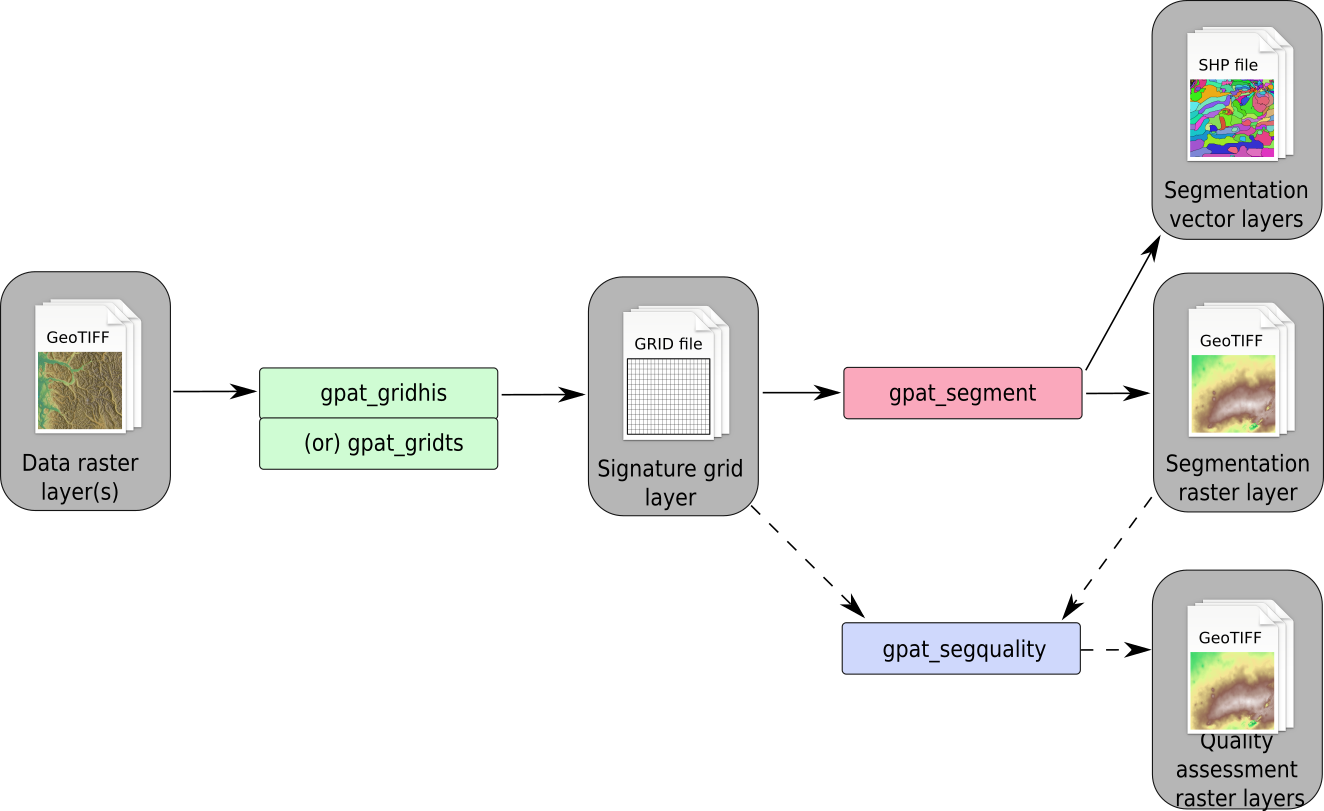
\includegraphics[width=\textwidth]{segment_scheme.png}
	\caption{Workflow path for segmentation.}
	\label{FIG:SEGMENT}
\end{figure}

\FloatBarrier

\subsection{Clustering}
TODO

\subsubsection{Clustering of individual motifels}

\begin{figure}[H]
	\centering
	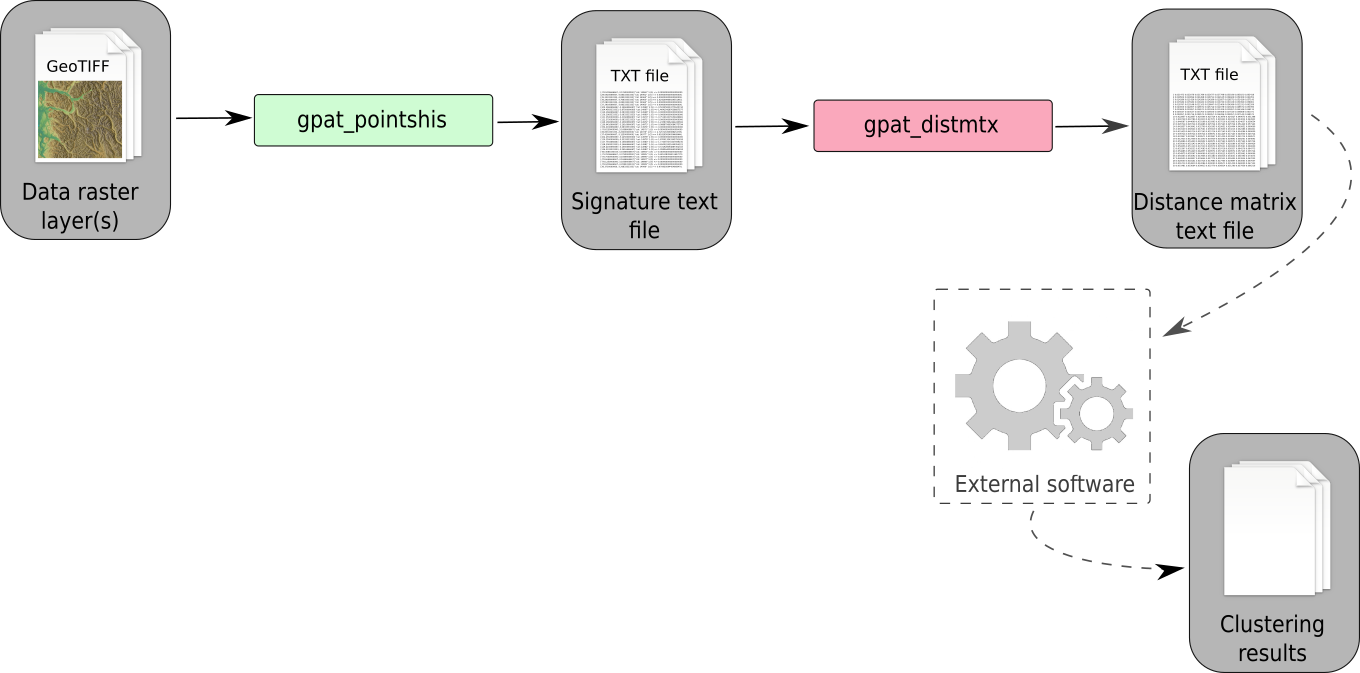
\includegraphics[width=\textwidth]{cluster_points_scheme.png}
	\caption{Workflow path for clustering of motifels.}
	\label{FIG:CLUSTER_POINTS}
\end{figure}

\begin{figure}[H]
	\centering
	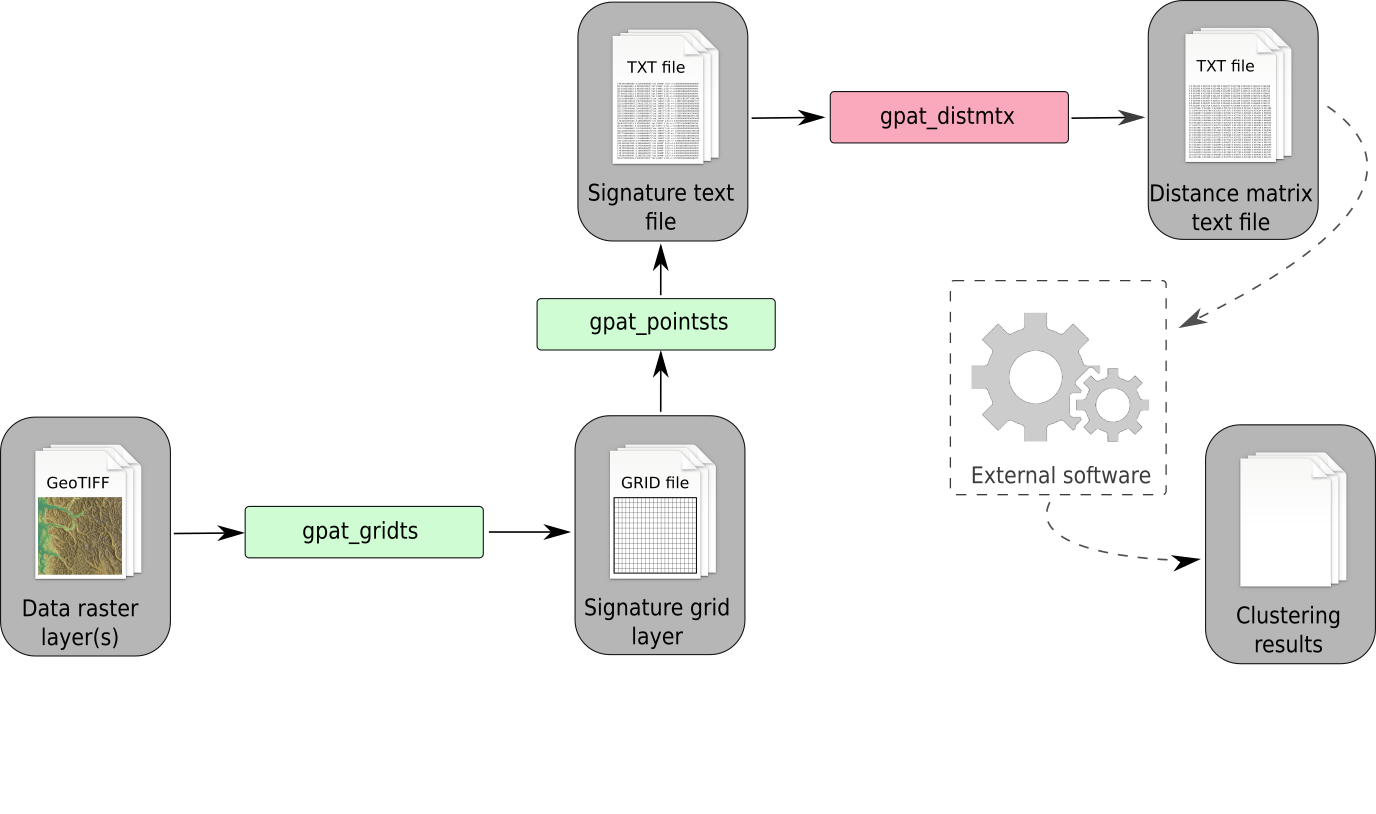
\includegraphics[width=\textwidth]{cluster_pointsts_scheme.png}
	\caption{Workflow path for clustering of time series motifels.}
	\label{FIG:CLUSTER_POINTSTS}
\end{figure}

\FloatBarrier

\subsubsection{Clustering of grid of motifels}

\begin{figure}[H]
	\centering
	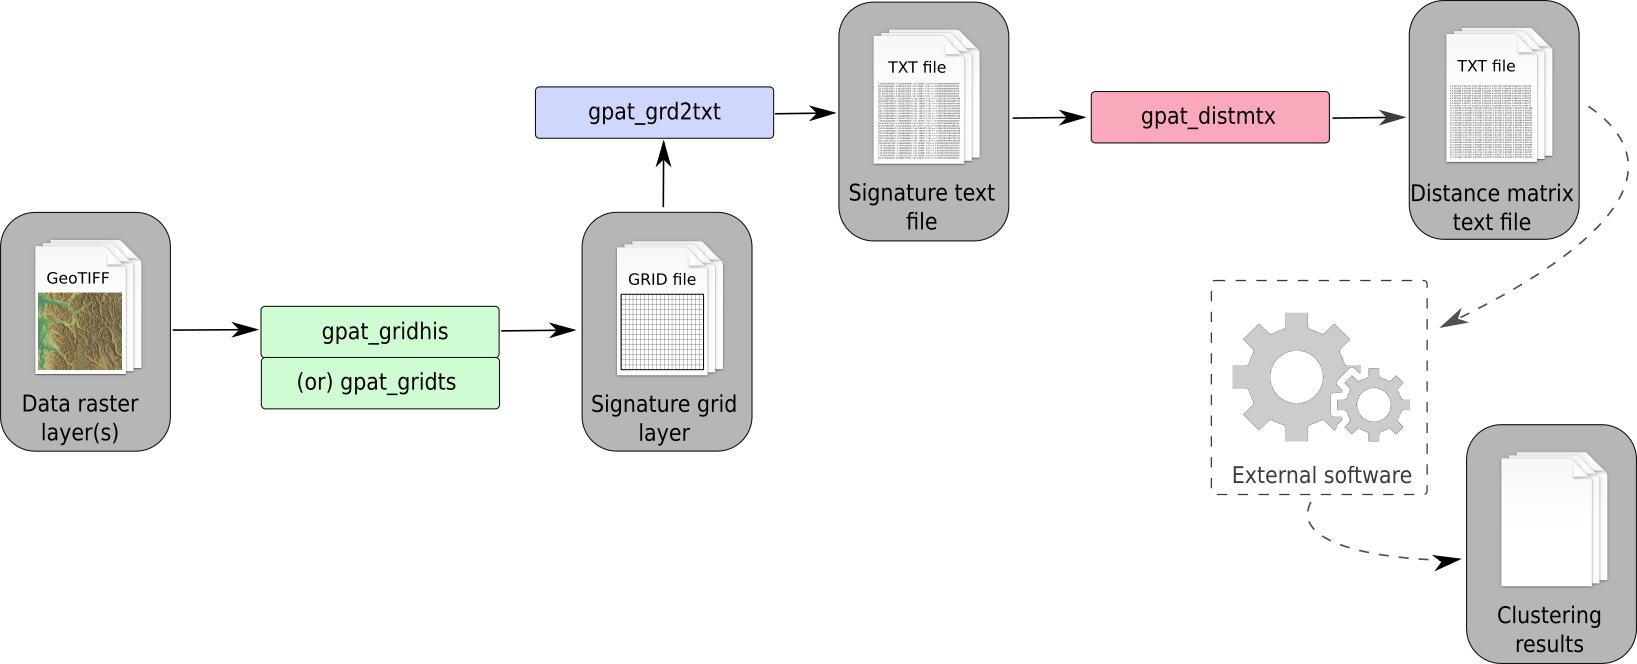
\includegraphics[width=\textwidth]{cluster_grid_scheme.png}
	\caption{Workflow path for clustering of grid of motifels.}
	\label{FIG:CLUSTER_GRID}
\end{figure}

\FloatBarrier

\subsubsection{Clustering of segments/predefined irregular regions}

\begin{figure}[H]
	\centering
	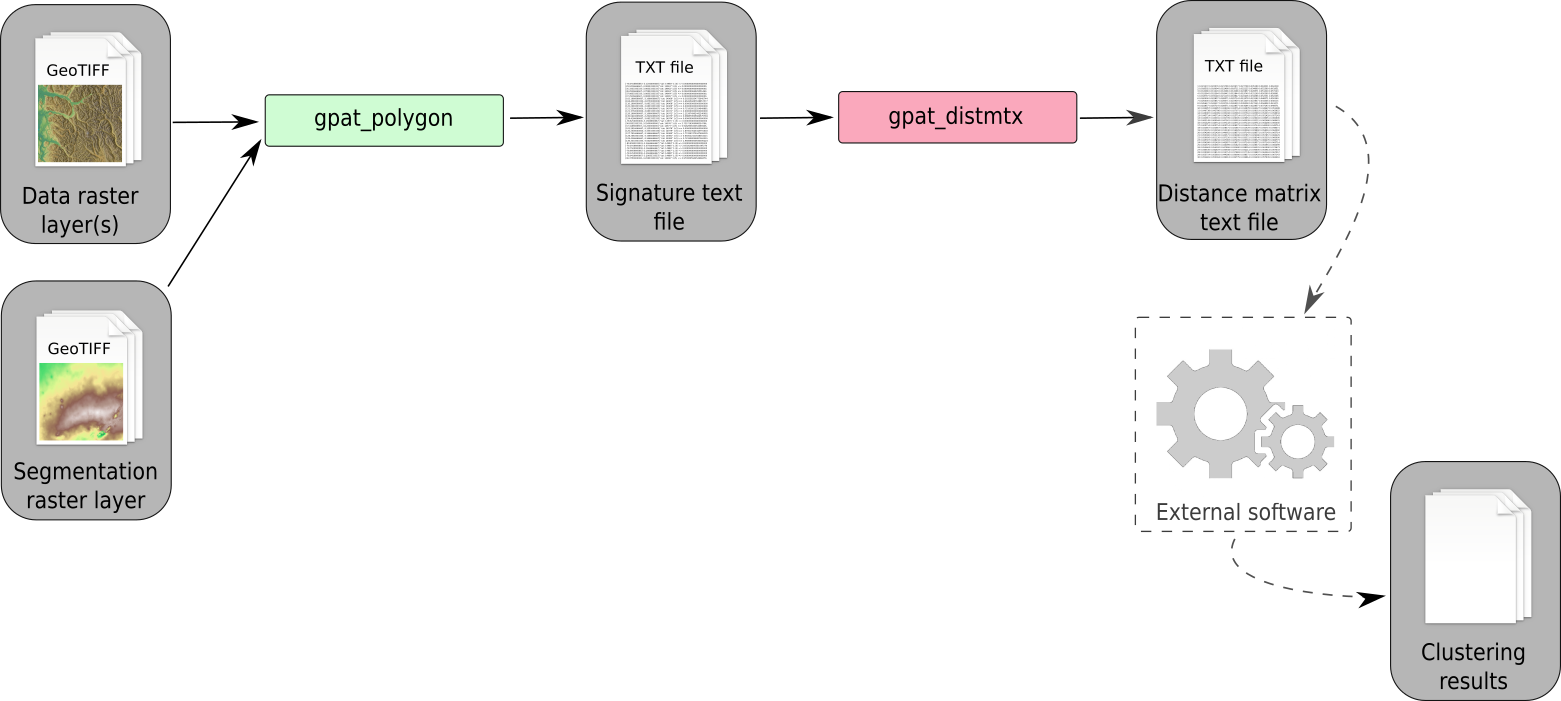
\includegraphics[width=\textwidth]{cluster_seg_scheme.png}
	\caption{Workflow path for clustering of segments (regions).}
	\label{FIG:CLUSTER_SEGMENT}
\end{figure}